%%
%% This is file `squelette-rr.tex',
%% generated with the docstrip utility.
%%
%% The original source files were:
%%
%% RR.dtx  (with options: `sample')
%% ********************************************************************
%% Copyright (C) 1997-1999 2004 2006-2011 INRIA/APICS/MARELLE by Jose' Grimm
%% This file may be distributed and/or modified under the
%% conditions of the LaTeX Project Public License, either version 1.3
%% of this license or (at your option) any later version.
%% The latest version of this license is in
%%    http://www.latex-project.org/lppl.txt
%% and version 1.3 or later is part of all distributions of LaTeX
%% version 2003/12/01 or later.
%% An archive of the software can be found at
%%    ftp://ftp-sop.inria.fr/marelle/RR-INRIA

\documentclass[twoside]{article}
\usepackage[a4paper]{geometry}
\usepackage[latin1]{inputenc} % ou \usepackage[utf8]{inputenc}
\usepackage[T1]{fontenc} % ou \usepackage[OT1]{fontenc}
\usepackage{RR}
\usepackage{hyperref}
\usepackage{subfigure}
%%\usepackage[frenchb]{babel} % optionnel
\RRNo{7003}
%% \RTNo{0703}
%%
%% date de publication du rapport
\RRdate{April 2015}
%%
%% Cas d'une version deux
%% \RRversion{2}
%% date de publication de la version 2
%% \RRdater{November 2008}
%%
\RRauthor{% les auteurs
 % Premier auteur, avec une note
H\'el\'ene Coullon\thanks{Footnote for first author}%
  % note partag\'ee (optionnelle)
  \thanks[sfn]{Shared foot note}%
 % \and entre chaque auteur s'il y en a plusieurs
  \and
Christian Perez\thanks{Footnote for second author}%
 % r\'ef\'erence \`a la note partag\'ee
%\thanksref{sfn}
 % liste longue pour tests de mise en page
%\and Nicolas Bourbaki\thanks{etc} \and Andr\'e Lichnerowicz
%\and Marcel-Paul Sch\"utzenberger \and Jacques-Louis Lions
}
%% Ceci apparait sur chaque page paire.
\authorhead{Coullon \& Perez}
%% titre francais long
\RRtitle{Exemple de document\\
 utilisant le style\\rapport de recherche\\Inria}
%% English title
\RRetitle{Component-based implicit parallelism model for multi-stencil numerical simulations}
%%
%\titlehead{Example of RR.sty}
%%
%\RRnote{This is a note}
%\RRnote{This is a second note}
%%
\RRresume{Resume en francais
}
\RRabstract{
abstract }
%%
\RRmotcle{mots-cles}
%%
%% \RRprojet{Apics}  % cas d'un seul projet
\RRprojets{Avalon}
%%
%% \URLorraine % pour ceux qui sont \`a l'est
%% \URRennes  % pour ceux qui sont \`a l'ouest
%\URRhoneAlpes % pour ceux qui sont dans les montagnes
%% \URRocq % pour ceux qui sont au centre de la France
%% \URFuturs % pour ceux qui sont dans le virtuel
%% \URSophia % pour ceux qui sont au Sud.
%%
%% \RCBordeaux % centre de recherche Bordeaux - Sud Ouest
%% \RCLille % centre de recherche Lille Nord Europe
%% \RCParis % Paris Rocquencourt
%% \RCSaclay % Saclay \^Ile de France
 \RCGrenoble % Grenoble - Rh\^one-Alpes
%% \RCNancy % Nancy - Grand Est
%% \RCRennes % Rennes - Bretagne Atlantique
%\RCSophia % Sophia Antipolis M\'editerran\'ee
\newtheorem{mydef}{\textbf{Definition}}
\usepackage{amsmath}
\usepackage{amssymb}
\usepackage{graphics}
\usepackage{tikz}
\usepackage[ruled,noend]{algorithm2e}
\usetikzlibrary{calc,arrows,shapes,automata,petri,positioning,decorations.markings,shadows}

\tikzset{
    component/.style={
    rectangle,rounded corners=3pt,draw=black
    },
    dcomponent/.style={
    rectangle,rounded corners=3pt,dashed,draw=black
    },
    smallcp/.style={
    rectangle,rounded corners=3pt,draw=black,font=\tiny,
    },
    resource/.style={
    rectangle,rounded corners=3pt, dashed,draw=black,font=\tiny,
    },
    connection/.style={
    decoration={ markings,
      mark=at position 1 with {\node[fill=black,draw=black,circle,inner sep=2pt](conn){};}
      },
    postaction={decorate}
    },
    bconnection/.style={
    decoration={ markings,
      mark=at position 1 with {\node[fill=black,draw=black,circle,inner sep=2pt](conn){};}
      },
    postaction={decorate}
    },
    mpiconn/.style={
    decoration={ markings,
      mark=at position 0.99 with {\node[fill=black,draw=black,rectangle,,inner sep=2pt](mpi){};}
      },
    postaction={decorate}
    },
}


%%
\begin{document}

%%
\makeRR   % cas d'un rapport de recherche
%% \makeRT % cas d'un rapport technique.
%% a partir d'ici, chacun fait comme il le souhaite

\tableofcontents

%------------------------------------------------------------------------------
\section{Introduction}
\label{sect:introduction}
%------------------------------------------------------------------------------
\section{Multi-stencil programs}
\label{sect:formalism}
To numerically solve a set of PDEs, iterative methods (finite difference, finite volume or finite element methods) are frequently used to approximate the solution through a discretized (step by step) phenomena. Thus, the continuous time and space domains are discretized so that a set of numerical computations are iteratively (time discretization) applied onto a mesh (space discretization). In other words, the PDEs are transformed to a set of numerical computations applied at each time step on all elements of the discretized space domain. Among those numerical computations is found a set of numerical schemes, also called \textit{stencil computations}, and a set of auxiliary computations also needed to perform the simulation, and also called \emph{local computations}.
This section gives formal definitions of a \textit{stencil program} and its computations. Then, the different parallelization techniques which can be applied on such program, are presented.

%-------------------------------------
\subsection{Time, mesh and data}

A mesh $\mathcal{M}$ defines the discretization of the continuous space domain $\Omega$ of a set of PDEs and is defined as followed. 

\begin{mydef}
\textit{A mesh is a connected undirected graph $\mathcal{M}=(V,E)$, where $V$ is the set of vertices and $E$ the set of edges. The set of edges $E$ of a mesh $\mathcal{M}=(V,E)$ does not contain bridges.}
\end{mydef}

\rmq{Pas très clair la suite; motivation? dom == some sub elements of M ?}
\begin{mydef}
$D_i$ is a set of elements of a mesh $\mathcal{M}=(V,E)$, constructed by a function $dom_i$ which defines a precise association between $V$ and $E$, $dom_i : V \times E \rightarrow D_i$.
\end{mydef}
For example, the set of cells $D_0$ in a Cartesian 2D mesh could be defined by exactly four vertices and four edges connected as a cycle. But we could also define another set of elements $D_1$ as the simple set of vertices $V$, etc.

A mesh can be structured (as Cartesian or curvilinear meshes), unstructured, regular or irregular (without the same topology for each element) and hybrid. 

\begin{figure}[!h]\begin{center}
  \resizebox{8cm}{!}{\includegraphics{./images/maillages.pdf}}
  \caption{From left to right, Cartesian, curvilinear and unstructured meshes.}
  \label{fig:mesh}
\end{center}\end{figure}

\begin{mydef}
The discretization of the continuous time domain $\mathcal{T}$ is denoted $T$ such that $\forall\mbox{ }t_i\mbox{, }t_{i+1} \in T\mbox{, }\exists\mbox{ }\Delta t \in \mathbb{R}$\mbox{, }$t_{i+1} = t_i + \Delta t$. Thus, $T$ is responsible for the iteration time steps of the numerical simulation. 
\end{mydef}

In a numerical simulation a set of data, or quantities, are applied onto the mesh and represent the set of values to compute, or to use, for computation.

\begin{mydef}
The set of data applied on the mesh is denoted by $\Delta$, such that $\delta \in \Delta$ is a function which associates each element $d \in D_i$ (the domain it is applied on) to a value $v \in V$, $\delta : D_i \rightarrow V$. In the rest of this paper, the domain of a data $\delta$ can be given by the function $domain(\delta)=D_i$.
\end{mydef}
One can notice that in applied mathematics, the signature of $\delta$ would be $\delta : D_i \times T \rightarrow V$, however when programming a numerical simulation it is not wise to store all values of each time iteration.

%-----------------------
\subsection{Computations}

\begin{mydef}
A numerical expression $\text{exp}$ is a function which represents how to compute a value for an element $d \in domain(w)=D_i$, using the set $R \subset \Delta$ of input data (read data), $\text{exp} : R \times D_i \rightarrow w \times D_i$.
\end{mydef}

\begin{mydef}
A computation $c$ of a numerical simulation is defined as $c(R,w,\text{exp})$, where $R \subset \Delta, w \in \Delta$ and $\text{exp}$ a numerical expression. %$D$ is one of the subsets $D_i \subset \mathcal{M}$, such that $w : D \rightarrow V$.
\end{mydef}
It has to be noticed that at each time iteration, all the elements of a mesh are computed. However, it happens that computations of the mesh elements are splitted in different domains, as for example the computation of the physical border. In this case additional $D_i$ can be specified for the mesh $\mathcal{M}$.

\begin{mydef}
The set of $n$ ordered computations of a numerical simulation is denoted $\Gamma = [c_i]_{0 \leq i \leq n-1}$, such that $\forall c_i,c_j \in \Gamma$, if $i \leq j$, then $c_i$ is computed before $c_j$, and $c_j$ can be computed only when $c_i$ is finished.
\end{mydef}

\begin{mydef}
A \textit{multi-stencil program} is defined by the quadruplet $\mathcal{MSP}(T,\mathcal{M},\Delta,\Gamma)$.
\end{mydef}
%If the number of computations in $\Gamma$ is $card(\Gamma)=n$, such that $\bigcup_{i=0}^{n-1}c_i = \Gamma$, then $\bigcup_{i=0}^{m-1}R_i \cup w_i \subseteq \Delta$.

As already mentioned, the ordered list $\Gamma$ can be composed of two different types of computations, stencil and local computations, which will be defined in the rest of this Section.

\begin{mydef}
The neighborhood $\mathcal{N}$ of an element $d \in D_i$ is a function to obtain a set of elements in any $D_k \subset \mathcal{M}$, $\mathcal{N} : D_i \rightarrow D_k \times D_k \times \dots$.
\end{mydef}
The function $\mathcal{N}$ is also sometimes called the \textit{stencil shape}, or the \textit{stencil} in applied mathematics. In this paper we distinguish a stencil shape from a \textit{stencil computation} defined as followed:

\begin{mydef}
A \textit{stencil computation} is defined as a quadruplet $s(R,w,\text{exp},\mathcal{N})$, where $R \subset \Delta$, and $w : D \rightarrow V \in \Delta$.
\end{mydef}
In a stencil computation $s$, $\forall d \in D$, the stencil numerical expression $\text{exp}$ is applied such that $w(d) = \text{exp}(R(d),R(\mathcal{N}(d))$. In this work, a stencil computation $s(R,w,\text{exp},\mathcal{N})$ always verifies $R \cap \{w\} = \emptyset$, otherwize an implicit numerical scheme has to be solve which is over the scope of this paper. As a result, the ordered list $\Gamma$ of a multi-stencil program can be composed of a set of stencil computations applied on one or more stencil shapes.

Figure~\ref{fig:ex} gives an example of a stencil computation $s(R,w,\text{exp},\mathcal{N})$, where $\mathcal{M}(V,E)$ is a two dimensional Cartesian mesh. A single domain $D=domain(w)$ is defined in this example and is composed of cells formed by a cycle of four vertices $v \in V$ and four edges $e \in E$. Furthermore, in this example $R=\{A\}$, $w=B$, and for $(x,y) \in D$ the neighborhood function is 
\begin{equation*}
\mathcal{N} : (x,y) \rightarrow \{(x,y+1),(x,y-1),(x+1,y),(x-1,y)\}.
\end{equation*}
Finally, the numerical expression of this example is 
\begin{equation*}
\text{exp}(A(x,y),A(\mathcal{N}(x,y)) = B(x,y) = A(x,y)+(A(x,y+1)+A(x,y-1)+A(x+1,y)+A(x-1,y))/4.
\end{equation*}

\begin{figure}[!h]\begin{center}
  \resizebox{8cm}{!}{\includegraphics{./images/example.pdf}}
  \caption{Example of a stencil computation.}
  \label{fig:ex}
\end{center}\end{figure}

The second type of numerical computation is a local computation.
\begin{mydef}
A local computation is a triplet $l(R,w,\text{exp})$, where $exp$ does not involve a neighborhood function $\mathcal{N}$.
\end{mydef}

A stencil program and stencil and local computations have been formally defined in this section. This formalism is used in the next Section to define two parallelization techniques of a multi-stencil program.



%------------------------------------------------------------------------------
\section{Component-based parallelism model}
\label{sect:component}
%-------------------------------------
\subsection{Component models}
A \textit{component} is an independent object which represents a functionnality of an application, and which is associated to a set of \textit{interfaces} used to plug an instance of a component with other ones. The object composed of multiple component instances linked together through their interfaces is called a component assembly. As a result, a component assembly is the code of an entire application represented as a set of splitted functionnalities. Such software engineering model is known to increase \textit{code re-use} and \textit{productivity}, as one component can be used in different applications, but also \textit{maintainability} and \textit{scalability}, as functionnalities of an application are clearly splitted in different and independent components. More recently, component models have been studied to write HPC applications such as $L^2C$~\cite{} (Low Level Component Model) and CCA~\cite{} (Common Component Architecture).

In the rest of this paper, the component model $L^2C$ is considered and used by the solution. A component is defined as
\begin{equation}
C(I,F),
\end{equation}
where $I$ is a set of available interfaces for the given component, and $F$ is the set of functions to answer the functionnality of the component. A component instance, as for an object, is the actual creation of the component, and more than one instance can be created. The components of $L^2C$ are limited to a few interfaces without the introduction of overheads. In this paper we are interested in four types of interfaces. The three first one are \textit{use} and \textit{provide} interfaces (Figure~\ref{AB}) to use a functionnality provided by another component instance, and \textit{use-multiple} interface (Figure~\ref{ABC}) to use a vector of functionnalities provided by a set of component instances. A condensed notation of a use-multiple is given in the Figure~\ref{ABCbis}. 

\begin{figure}[h!]
\begin{center}
  \subfigure[][$A$ uses $B$ and $A$ uses $C$]{
  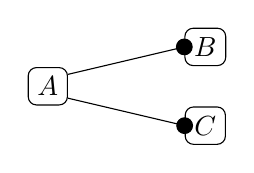
\begin{tikzpicture}[shorten >=1pt, node distance=2cm, on grid, auto]
   \node[component] (A) at (0,0) {$A$};
   \node[component] (B) at (2,+0.5) {$B$};
   \node[component] (C) at (2,-0.5) {$C$};
 
  \path[-]
    ([yshift=1ex]A.east) edge [connection] (B.west)
    ([yshift=-1ex]A.east) edge [connection] (C.west);
  \end{tikzpicture}
  \label{AB}
  }
  \hspace{2cm}
  \subfigure[][$A$ uses multiple $B$ instances]{
  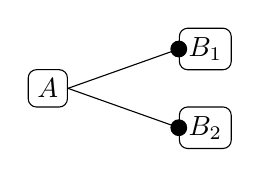
\begin{tikzpicture}[shorten >=1pt, node distance=2cm, on grid, auto]
   \node[component] (A) at (0,0) {$A$};
   \node[component] (B) at (2,+0.5) {$B_1$};
   \node[component] (C) at (2,-0.5) {$B_2$};
 
  \path[-]
    (A.east) edge [connection] node {} (B.west)
             edge [connection] node {} (C.west);

  \end{tikzpicture}
  \label{ABC}
  }
  \hspace{2cm}
  \subfigure[][$A$ uses multiple $B$ instances (condensed notation)]{
  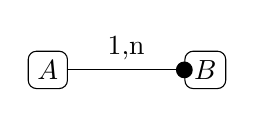
\begin{tikzpicture}[shorten >=1pt, node distance=2cm, on grid, auto]
   \node[component] (A) at (0,0) {$A$};
   \node[component] (B) at (2,0) {$B$};
 
  \path[-]
    (A.east) edge [connection] node {1,n} (B.west);

  \end{tikzpicture}
  \label{ABCbis}
  }
  \caption{$L^2C$ use-provide and use-multiple interfaces}
  \label{interfaces}
\end{center}
\end{figure}

An instance $i$ of a component has the same properties than the component it is instanciated from, but it is also asociated to a resource $r$ (a core, a thread etc.) of the set of all available resources $R$.
\begin{equation}
C_i(I,F,r)
\end{equation}
A component assembly represents the application as a set of component instances and the composition of those instances through their interfaces. A component assembly is defined as
\begin{equation}
\alpha (\mathcal{C},L,R),
\end{equation}
where $\mathcal{C}$ is the set of component instances used, $L$ is the set of links between interfaces of component instances, and $R$ is the set of available resources. The component assembly of $L^2C$ offers a way to write an assembly for each MPI process, and to connect some of their components by MPI communicators. This connection is an \textit{MPI interface}. In the rest of this paper we consider a broader interface called \textit{synchronization}, which corresponds to the MPI interface of $L^2C$ but which could also be a \textit{thread synchronization} instead.

Using those four interfaces (use, use-multiple, provide and synchronization), it is possible to write an application with medium-grain components, enough fine to keep efficiency and to stay close to the execution model, and enough coarse to take advantage of components. The efficiency of $L^2C$ has been proved, while increasing the productivity and maintainability of HPC applications, but moreover it has also been shown that the protability of such component-based HPC application is improved~\cite{}.

%-------------------------------------
\subsection{Stencil program parallelization using components}
In this section is studied the parallelization of a numerical simulation using the given definitions of a component, an assembly and four interfaces. First, the different parallelization techniques explained in the Section~\ref{sect:parall} are translated to component-based parallel assemblies, and an approximation of the general case is discussed for the solution presented in this paper. In the rest of this section, the following example of dependencies is used 
\begin{equation}
A<((B<D) \parallel C)<E \ll A'<((B'<D') \parallel C'),
\label{eq:dep}
\end{equation}
 where $A,B,C,D,E,A',B',C',D'$ are numerical computations. %In this example, $\parallel$ is a binary expression which means that a parallel execution of the right and left computations is possible. It is equivalent to $\not>$. 
This example, can be represented as a directed acyclic graph as in the Figure~\ref{example}.

\begin{figure}[h!]
\begin{center}
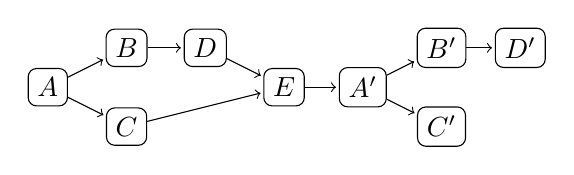
\begin{tikzpicture}[shorten >=1pt, node distance=2cm, on grid, auto]
   \node[component] (A) at (0,0) {$A$};
   \node[component] (B) at (1,+0.5) {$B$};
   \node[component] (C) at (1,-0.5) {$C$};
   \node[component] (D) at (2,+0.5) {$D$};
   \node[component] (E) at (3,0) {$E$};
   \node[component] (AA) at (4,0) {$A'$};
   \node[component] (BB) at (5,+0.5) {$B'$};
   \node[component] (CC) at (5,-0.5) {$C'$};
   \node[component] (DD) at (6,+0.5) {$D'$};
 
  \path[->]
    (A) edge node {} (B)
        edge node {} (C)
    (B) edge node {} (D)
    (D) edge node {} (E)
    (C) edge node {} (E)
    (E) edge node {} (AA)
    (AA) edge node {} (BB)
        edge node {} (CC)
    (BB) edge node {} (DD);
  \end{tikzpicture}
  \caption{Dependencies example~(\ref{eq:dep}) represented as a DAG.}
  \label{example}
\end{center}
\end{figure}

%---------
%---------
\paragraph{Coarse- and fine-grain data parallelism.} 
As explained in the Section~\ref{sect:parall}, to apply coarse-grain data parallelism on numerical simulations, a domain decomposition (or graph partitioning) has to be done on the mesh and also on the data mapped on it. When this important step is solved, the same program can be applied on each subpart of the data, on the different resources. In addition to this, a set of synchronizations are needed between the resources at each time step to compute the neighborhood $\mathcal{N}$ correctly. When using a component model, the computing part of the application, which is called for each time step, can be seen as a component assembly which is duplicated on different resources, which is possible using $L^2C$ for example. However, it is needed to classify computations in the component assembly to identify when synchronizations are needed (denoted $\ll$ in the Section~\ref{sect:dep}). For this reason, a \textit{sequence} component $SEQ$, which uses one after the other a set of computation components, is defined as 
\begin{equation}
SEQ(\{provide,use-multiple\},\{sequence\}).
\end{equation} 
Thus, the \textit{sequence} function (represented in the Algorithm~(\ref{alg:seq})) is responsible for the loop which calls as much \textit{uses} as the number of components connected to the \textit{use-multiple}. In addition to this, a \textit{synchronized sequence} component $SSEQ$, which uses one after the other a set of computation components, but which also proceeds synchronizations between them, is defined as 
\begin{equation}
SSEQ(\{provide,use-multiple, synchronization\},\{ssequence\}).
\end{equation}
In this case, the \textit{ssequence} function (represented in the Algorithm~(\ref{alg:sseq})) is responsible for a loop of two steps, first a synchronization step, second a use step. Finally, each numerical computation is represented by a component 
\begin{equation}
K(\{provide\},\{compute\}),
\end{equation}
 where the function \textit{compute} (represented in the Algorithm~(\ref{alg:comp})) is responsible for the sapce loop and the numerical computation on each element of the mesh.

\begin{center}
\begin{minipage}[t]{7cm}
  \vspace{0pt} 
 \begin{algorithm}[H]
 \ForAll{component $cp$ to use}{
 use the provide interface of $cp$
 }
 \caption{sequence function}
 \label{alg:seq}
 \end{algorithm}
 \end{minipage}%
 \hspace{0.5cm}
\begin{minipage}[t]{7cm}
  \vspace{0pt}
 \begin{algorithm}[H]
 \ForAll{component $cp$ to use}{
 synchronizations\\
 use the provide interface of $cp$
 }
 \label{alg:sseq}
 \caption{ssequence function}
 \end{algorithm}
 \end{minipage}%
\end{center}

%\begin{minipage}[t]{5cm}
 % \vspace{0pt}
 \begin{center}
 \begin{algorithm}[H]
 \ForAll{elements $d$ in $D$}{
 $w(d)=e(R(d),R(\mathcal{N}(d)))$
 }
 \caption{compute function}
 \label{alg:comp}
 \end{algorithm}
 \end{center}
%\end{minipage}%
Using the three components $SSEQ$, $SEQ$, and $K$, the component assembly of the dependencies~(\ref{eq:dep}) is represented in the Figure~~\ref{exdataparall}. One can notice, in this Figure, that the parallel dependencies ($\parallel$) are lost. However, in a SPMD parallelization, the parallelism is obtained from executing the same program on different part of the data. As a result, a correct sequence of computations is sufficient to expose coarse-grain data parallelism.
%---------
\begin{figure}[h!]
\begin{center}
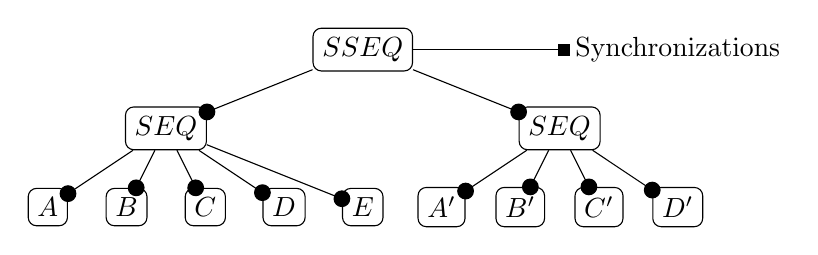
\begin{tikzpicture}[shorten >=1pt, node distance=2cm, on grid, auto]
  \node[component] (SSEQ) at (0,0) {$SSEQ$};
  \node (sync) at (4,0) {Synchronizations};
  \node[component] (SEQ1) at (-2.5,-1) {$SEQ$};
  \node[component] (SEQ2) at (2.5,-1) {$SEQ$};
  \node[component] (A) at (-4,-2) {$A$};
  \node[component] (B) at (-3,-2) {$B$};
  \node[component] (C) at (-2,-2) {$C$};
  \node[component] (D) at (-1,-2) {$D$};
  \node[component] (E) at (0,-2) {$E$};
  \node[component] (AA) at (1,-2) {$A'$};
  \node[component] (BB) at (2,-2) {$B'$};
  \node[component] (CC) at (3,-2) {$C'$};
  \node[component] (DD) at (4,-2) {$D'$};
 
  \path[-]
    (SSEQ) edge [connection] node {} (SEQ1)
           edge [connection] node {} (SEQ2)
           edge [mpiconn] node {} (sync)
    (SEQ1) edge [connection] node {} (A)
           edge [connection] node {} (B)
           edge [connection] node {} (C)
           edge [connection] node {} (D)
           edge [connection] node {} (E)
    (SEQ2) edge [connection] node {} (AA)
           edge [connection] node {} (BB)
           edge [connection] node {} (CC)
           edge [connection] node {} (DD);

  \end{tikzpicture}
\caption{Example assembly for coarse- and fine-grain data parallelism}
\label{exdataparall}
\end{center}
\end{figure}
The overall computation assembly of an SPMD numerical simulation is composed of a duplication of the computation (or dependencies) assembly described above. Each duplication is applied on an available resource as illustrated in the Figure~\ref{overall}. In the rest of this paper, this overall computation assembly of an SPMD application (coarse-grain data parallelism) is represented as a single computation assembly, and the $SSEQ$ component indicate where the synchronizations are needed.

%---------
\begin{figure}[h!]
\begin{center}
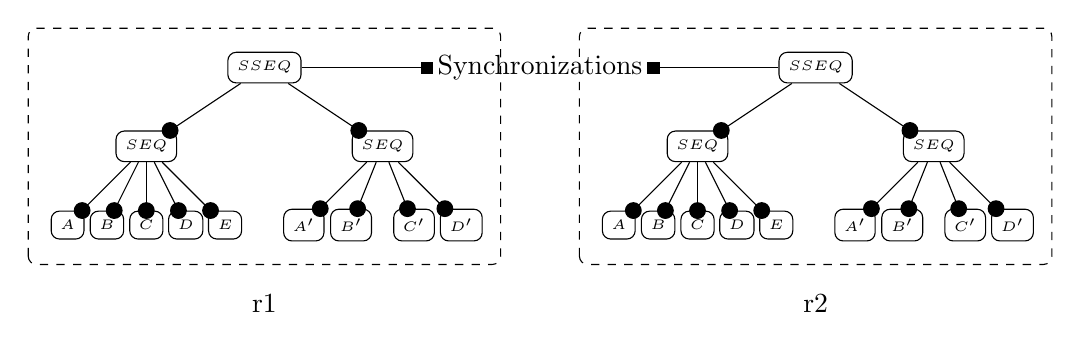
\begin{tikzpicture}[shorten >=1pt, node distance=2cm, on grid, auto]
  \node[smallcp] (SSEQ) at (0,0) {$SSEQ$};
  \node (sync) at (3.5,0) {Synchronizations};
  \node[smallcp] (SEQ1) at (-1.5,-1) {$SEQ$};
  \node[smallcp] (SEQ2) at (1.5,-1) {$SEQ$};
  \node[smallcp] (A) at (-2.5,-2) {$A$};
  \node[smallcp] (B) at (-2,-2) {$B$};
  \node[smallcp] (C) at (-1.5,-2) {$C$};
  \node[smallcp] (D) at (-1,-2) {$D$};
  \node[smallcp] (E) at (-0.5,-2) {$E$};
  \node[smallcp] (AA) at (0.5,-2) {$A'$};
  \node[smallcp] (BB) at (1.1,-2) {$B'$};
  \node[smallcp] (CC) at (1.9,-2) {$C'$};
  \node[smallcp] (DD) at (2.5,-2) {$D'$};
  \draw [resource] (-3,-2.5) rectangle +(6cm, 3cm);
  \node (R1) at (0,-3) {r1};

  \node[smallcp] (SSEQ2) at (7,0) {$SSEQ$};
  \node[smallcp] (SEQ3) at (5.5,-1) {$SEQ$};
  \node[smallcp] (SEQ4) at (8.5,-1) {$SEQ$};
  \node[smallcp] (A2) at (4.5,-2) {$A$};
  \node[smallcp] (B2) at (5,-2) {$B$};
  \node[smallcp] (C2) at (5.5,-2) {$C$};
  \node[smallcp] (D2) at (6,-2) {$D$};
  \node[smallcp] (E2) at (6.5,-2) {$E$};
  \node[smallcp] (AA2) at (7.5,-2) {$A'$};
  \node[smallcp] (BB2) at (8.1,-2) {$B'$};
  \node[smallcp] (CC2) at (8.9,-2) {$C'$};
  \node[smallcp] (DD2) at (9.5,-2) {$D'$};
  \draw [resource] (4,-2.5) rectangle +(6cm, 3cm);
  \node (R2) at (7,-3) {r2};
 
  \path[-]
    (SSEQ) edge [connection] node {} (SEQ1)
           edge [connection] node {} (SEQ2)
           edge [mpiconn] node {} (sync)
    (SEQ1) edge [connection] node {} (A)
           edge [connection] node {} (B)
           edge [connection] node {} (C)
           edge [connection] node {} (D)
           edge [connection] node {} (E)
    (SEQ2) edge [connection] node {} (AA)
           edge [connection] node {} (BB)
           edge [connection] node {} (CC)
           edge [connection] node {} (DD)
    (SSEQ2) edge [connection] node {} (SEQ3)
           edge [connection] node {} (SEQ4)
           edge [mpiconn] node {} (sync)
    (SEQ3) edge [connection] node {} (A2)
           edge [connection] node {} (B2)
           edge [connection] node {} (C2)
           edge [connection] node {} (D2)
           edge [connection] node {} (E2)
    (SEQ4) edge [connection] node {} (AA2)
           edge [connection] node {} (BB2)
           edge [connection] node {} (CC2)
           edge [connection] node {} (DD2);

  \end{tikzpicture}
\caption{Overall SPMD computation assembly of the example~(\ref{eq:dep}) on two resources.}
\label{overall}
\end{center}
\end{figure}

But the assembly obtained from the instanciation of $SEQ$, $SSEQ$, and $K$ does not only expose coarse-grain data parallelism. Actually, the generic notation of a computation component $K$, which represents a numerical computation, is important to identifiy the different computations of a numerical simulation as different functionnalities of the program, but in addition to this, exposing a computation as a component, also exposes the fine-grain data parallelism level. In fact, a numerical computation is nothing more than a loop (or a nested loop) on the mesh elements and a numerical expression to compute (Algorithm~(\ref{alg:comp})). As a result a computation component is ideal to introduce SIMD and SIMT parallelism.

The general case of assembly to introduce coarse- and fine-grain data parallelism in numerical simulations is represented in the Figure~\ref{dataparall}.

\begin{figure}[h!]
\begin{center}
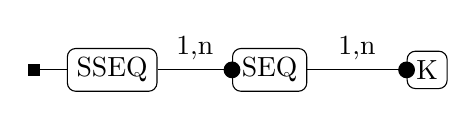
\begin{tikzpicture}[shorten >=1pt, node distance=2cm, on grid, auto]
   \node[component] (SSEQ) at (0,0) {SSEQ};
   \node[component] (SEQ) [right=of SSEQ] {SEQ};
   \node[component] (K) [right=of SEQ] {K};
 
  \path[-]
    (SSEQ)  edge [connection] node {1,n} (SEQ)
            edge [mpiconn] node {} (-1,0)
    (SEQ)	 edge [connection] node {1,n}	(K);
\end{tikzpicture}
\caption{General assembly description for coarse- and fine-grain data parallelism}
\label{dataparall}
\end{center}
\end{figure}
%---------

%---------
%---------
\paragraph{Data and task parallelism}
As also explained in the Section~\ref{sect:parall}, to apply task parallelism to numerical simulations, it is needed to identify the different tasks of the application and their dependencies. With the introduction of $SSEQ$, $SEQ$, and $K$ components, a part of this work is already done. Actually, each computation component $K$ represents a task. However, to be able to express all dependencies between computations, the $PAR$ component is defined as 
\begin{equation}
PAR(\{provide,use-multiple\},\{parallel\}),
\end{equation}
 and corresponds to the expression $\parallel$ or $\not<$. The function $parallel$ creates a thread for each component to use and join all threads at the end.

\begin{algorithm}[H]
 \ForAll{component $cp$ to use}{
 create thread $t$
 $t$ uses the provide interface of $cp$
 }
 join all threads
 \label{alg:par}
 \caption{parallel function}
 \end{algorithm}

\medskip
In addition to this, a composition of the components $SSEQ$, $SEQ$, $PAR$ and $K$ is needed to be able to represent complex dependencies. For example, the example dependencies~(\ref{eq:dep}) is represented in the Figure~\ref{exallparall}.
%---------
\begin{figure}[h!]
\begin{center}
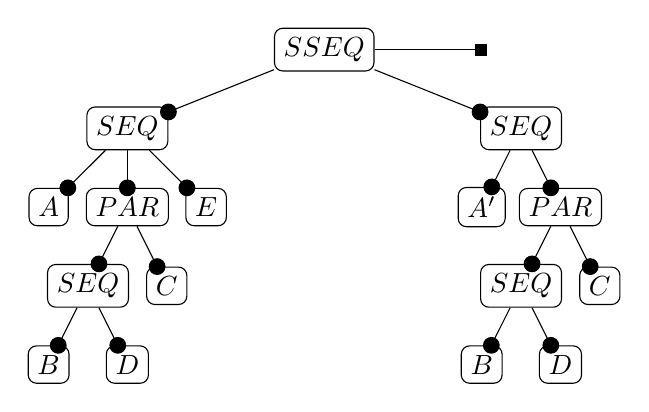
\begin{tikzpicture}[shorten >=1pt, node distance=2cm, on grid, auto]
  \node[component] (SSEQ) at (0,0) {$SSEQ$};
  \node[component] (SEQ1) at (-2.5,-1) {$SEQ$};
  \node[component] (SEQ2) at (2.5,-1) {$SEQ$};
  \node[component] (A) at (-3.5,-2) {$A$};
  \node[component] (E) at (-1.5,-2) {$E$};
  \node[component] (PAR1) at (-2.5,-2) {$PAR$};
  \node[component] (AA) at (2,-2) {$A'$};
  \node[component] (PAR2) at (3,-2) {$PAR$};
  \node[component] (SEQ3) at (-3,-3) {$SEQ$};
  \node[component] (C) at (-2,-3) {$C$};
  \node[component] (SEQ4) at (2.5,-3) {$SEQ$};
  \node[component] (CC) at (3.5,-3) {$C$};
  \node[component] (B) at (-3.5,-4) {$B$};
  \node[component] (D) at (-2.5,-4) {$D$};
  \node[component] (BB) at (2,-4) {$B$};
  \node[component] (DD) at (3,-4) {$D$};
 
  \path[-]
    (SSEQ) edge [connection] node {} (SEQ1)
           edge [connection] node {} (SEQ2)
           edge [mpiconn] node {} (2,0)
    (SEQ1) edge [connection] node {} (A)
           edge [connection] node {} (PAR1)
           edge [connection] node {} (E)
    (SEQ2) edge [connection] node {} (AA)
           edge [connection] node {} (PAR2)
    (PAR1) edge [connection] node {} (SEQ3)
           edge [connection] node {} (C)
    (PAR2) edge [connection] node {} (SEQ4)
           edge [connection] node {} (CC)
    (SEQ3) edge [connection] node {} (B)
           edge [connection] node {} (D)
    (SEQ4) edge [connection] node {} (BB)
           edge [connection] node {} (DD);

  \end{tikzpicture}
\caption{Example assembly for coarse- and fine-grain data parallelism}
\label{exallparall}
\end{center}
\end{figure}

The general case of assembly to introduce data parallelism and task parallelism in numerical simulations is represented in the Figure~\ref{allparall}.

%---------
\begin{figure}[h!]
\begin{center}
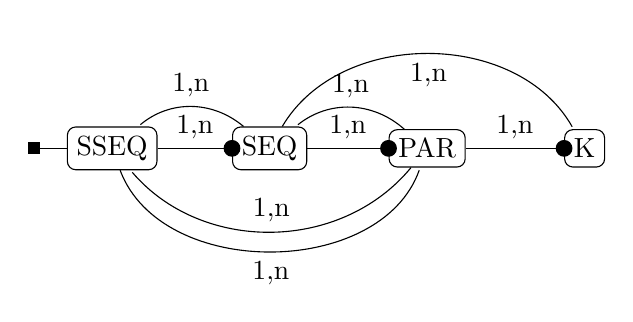
\begin{tikzpicture}[shorten >=1pt, node distance=2cm, on grid, auto]
   \node[component] (SSEQ) at (0,0) {SSEQ};
   \node[component] (SEQ) [right=of SSEQ] {SEQ};
   \node[component] (PAR) [right=of SEQ] {PAR};
   \node[component] (K)   [right=of PAR] {K};
 
  \path[-]
    (SSEQ)  edge  [bend right=70,connection] node  [swap] {1,n} (PAR)
    (SSEQ)  edge  [connection]                node          {1,n} (SEQ)
            edge  [mpiconn] node {} (-1,0)
    (SEQ)	  edge  [connection]                node          {1,n} (PAR)
    (PAR)   edge  [bend right=40,connection]  node  [swap]  {1,n} (SEQ)
    (SEQ)   edge  [bend right=40,connection]  node  [swap]  {1,n} (SSEQ)
    (PAR)   edge  [bend left=50,connection]   node  [swap]  {1,n} (SSEQ)
    (SEQ)   edge  [bend left=60,connection]   node  [swap]  {1,n} (K)
    (PAR)	  edge  [connection]                node          {1,n} (K);
\end{tikzpicture}
\caption{General assembly description for data and task parallelism}
\label{allparall}
\end{center}
\end{figure}
%---------

%---------
%---------
\paragraph{Intermediate expressivity}
The component assembly defined in the Figure~\ref{allparall} is usefull to expose data parallelism, task parallelism, and to have a complete expressivity for dependencies between computations. For the general case of scientific applications, this assembly is needed, however, this assembly has a certain number of drawbacks. First, $SSEQ$, $SEQ$ and $PAR$ do not represent functionnalities of the application but control of functionnalities. As a result, the role of a component is twisted. Second, in the case of a complex application, with complex dependencies, the component assembly is going to be riddled with $SSEQ$, $SEQ$ and $PAR$ components, making difficult the reading of the application. Thus, it decreases the maintainability bring by component models. Finally, this expressivity is as complex as a \textit{task graph}~\cite{}, and as a result, two additional difficulties get out if such an assembly is used in our solution: the automatic detection of complex dependencies from a simple description of the application, and the \textit{scheduling} of such tasks. This last point is particularly critical and difficult. Because of the compositions of $SSEQ$, $SEQ$ and $PAR$ components illustrated in the Figure~\ref{allparall}, and because of the definition of $PAR$ which simply creates a thread for each component to use, it is possible that the work of each thread becomes unbalanced. For example, the Figure~\ref{unbalanced} represents an unbalanced example. 

%---------
\begin{figure}[h!]
\begin{center}
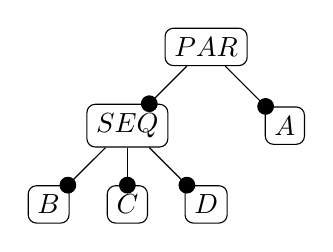
\begin{tikzpicture}[shorten >=1pt, node distance=2cm, on grid, auto]
  \node[component] (PAR1) at (0,0) {$PAR$};
  \node[component] (SEQ3) at (-1,-1) {$SEQ$};
  \node[component] (A) at (1,-1) {$A$};
  \node[component] (B) at (-2,-2) {$B$};
  \node[component] (C) at (-1,-2) {$C$};
  \node[component] (D) at (0,-2) {$D$};
 
  \path[-]
    (PAR1) edge [connection] node {} (SEQ3)
           edge [connection] node {} (A)
    (SEQ3) edge [connection] node {} (B)
           edge [connection] node {} (C)
           edge [connection] node {} (D);

  \end{tikzpicture}
\caption{Unbalanced assembly example}
\label{unbalanced}
\end{center}
\end{figure}

However, in existing component models for HPC (for exemple in $L^2C$) only the component object is defined, and all components are created, destroyed, and called the same way. Thus, it is not possible to manage a $PAR$ component to dynamically balance the workload on threads. For this reason, it seems that the combination of tasks and components are needed as well as a scheduler. The scheduling of a task graph is an active research domain and it could be an interesting perspective to work on the combination of $L^2C$ and StarPU~\cite{}, for example. However, this work aims to propose a light solution using component contributions, and to illustrate the advantages and drawbacks of such a solution. To only use components in our solution, and to avoid unbalanced and heavy assemblies, we propose an intermediate assembly which is an approximation of the general case of the Figure~\ref{allparall}. We claim, in the rest of this paper, that this approximation is enough expressive and produces efficient applications for the specific case of mesh-based numerical simulations.

The proposed intermediate assembly is represented in the Figure~\ref{approx}. The same basic association of components $SSEQ$, $SEQ$, $PAR$ and $K$ is found, however a limitation of the possible compositions of those components is applied. It is no longer possible to use a $SEQ$ or $SSEQ$ from a $PAR$ component, as well as using a $SSEQ$ from a $SEQ$ component and vice versa. The most important part of those limitations is to avoid too much imbalance. Actually, from a $PAR$ component it is only possible to use one computation $K$ in each created thread. In the specific case of mesh-based numerical simulations, as most numerical computations $c(R,w,D,e)$ (except boundary conditions) are applied on a complete set of mesh elements $D$ and computes a numerical expression $e$, two numerical computations are approximately balanced, or at least the imbalance is limited.

%If solving those problems for general cases seems needed in one hand (and this point is a perspective of this work), when focusing on mesh-based numerical simulations, such an expressivity is not essential on the other hand. To explain this claim, the Figure~\ref{approx} represents an approximation of the assembly of the Figure~\ref{allparall}. In this assembly, the available compositions are limited. Acually, a $SSEQ$ component exclusively uses multiple $SEQ$ components, which exclusively uses multiple $PAR$ or $K$. Finally, a $PAR$ component exclusively uses multiple $K$.

%---------
\begin{figure}[h!]
\begin{center}
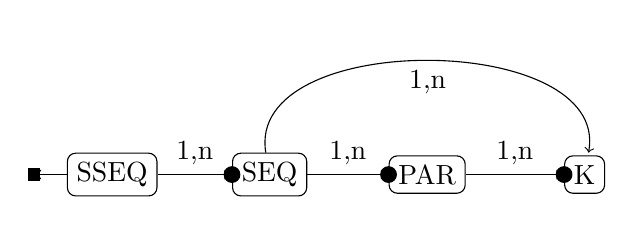
\begin{tikzpicture}[shorten >=1pt, node distance=2cm, on grid, auto]
   \node[component] (SSEQ) at (0,0) {SSEQ};
   \node[component] (SEQ) [right=of SSEQ] {SEQ};
   \node[component] (PAR) [right=of SEQ] {PAR};
   \node[component] (K) [right=of PAR] {K};
 
  \path[->]
             (SSEQ)  edge  [connection]               node           {1,n}   (SEQ)
                    edge [mpiconn] node {} (-1,0)
             (SEQ)   edge [connection]          node       {1,n}   (PAR)
             (SEQ)   edge [bend left=100,connection]   node  [swap]   {1,n}   (K)
             (PAR)   edge [connection]          node       {1,n}   (K);
\end{tikzpicture}
\caption{General assembly description approximation}
\label{approx}
\end{center}
\end{figure}

Using this approximated assembly, the assembly of the example is given in the Figure~\ref{exapprox}. The limitation of such an approximation is clearer in this example: the dependencies $(B<D) \parallel C$ and $(B'<D') \parallel C'$ can only be expressed by $B \parallel C<D$ which is a less precised dependency. But as explained before, this limitation of expressivity also guarantees a limitation of the imbalance which is due to the use of components only, and not task graphs and schedulers. Finally, the proposed approximation still exposes the three level of parallelism introduced in the Section~\ref{}.%When introducing task parallelism scheduling, this limitation can be a big disadvantage if the task (or functionnality) $B$ is short compared to $C$. However, in the case of a mesh-based numerical simulation, and as explained in the Section~\ref{sect:formalism}, most numerical computation $c(R,w,D,e)$ of a stencil program $\mathcal{P}(\mathcal{M},\Delta,\Gamma,\mathcal{T})$ are computed on all elements of $E_i \subset \mathcal{M}$, and computes a single numerical expression $e$. As a result most computations are close in terms of amount of numerical operations. Thus, thanks to the specific domain we are focussing on, the approximated assembly of the Figure~\ref{approx} is satisfactory and it makes the solution lighter by the only use of the component model $L^2C$, and without the need of an external task graph tool and scheduler. Finally, even if this assembly is an approximation of the real dependencies assembly, the three level of parallelism are still available in the solution.

%---------
\begin{figure}[h!]
\begin{center}
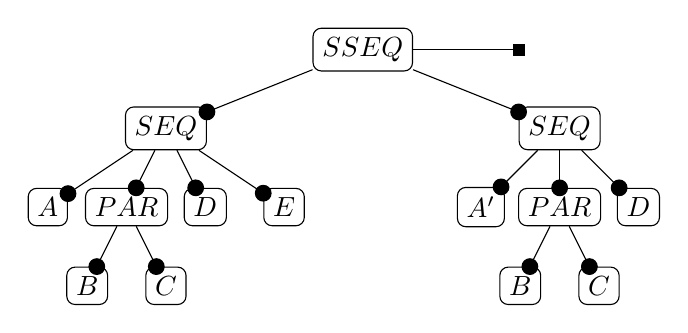
\begin{tikzpicture}[shorten >=1pt, node distance=2cm, on grid, auto]
  \node[component] (SSEQ) at (0,0) {$SSEQ$};
  \node[component] (SEQ1) at (-2.5,-1) {$SEQ$};
  \node[component] (SEQ2) at (2.5,-1) {$SEQ$};
  \node[component] (A) at (-4,-2) {$A$};
  \node[component] (PAR1) at (-3,-2) {$PAR$};
  \node[component] (D) at (-2,-2) {$D$};
  \node[component] (E) at (-1,-2) {$E$};
  \node[component] (AA) at (1.5,-2) {$A'$};
  \node[component] (PAR2) at (2.5,-2) {$PAR$};
  \node[component] (DD) at (3.5,-2) {$D$};
  \node[component] (B) at (-3.5,-3) {$B$};
  \node[component] (C) at (-2.5,-3) {$C$};
  \node[component] (BB) at (2,-3) {$B$};
  \node[component] (CC) at (3,-3) {$C$};
 
  \path[-]
    (SSEQ) edge [connection] node {} (SEQ1)
            edge [connection] node {} (SEQ2)
            edge [mpiconn] node {} (2,0)
    (SEQ1) edge [connection] node {} (A)
           edge [connection] node {} (PAR1)
           edge [connection] node {} (D)
           edge [connection] node {} (E)
    (SEQ2) edge [connection] node {} (AA)
           edge [connection] node {} (PAR2)
           edge [connection] node {} (DD)
    (PAR1) edge [connection] node {} (B)
           edge [connection] node {} (C)
    (PAR2) edge [connection] node {} (BB)
           edge [connection] node {} (CC);

  \end{tikzpicture}
\caption{Example assembly approximation}
\label{exapprox}
\end{center}
\end{figure}

%------------------------------------------------------------------------------
\section{Component Stencil Language}
\label{sect:csm}
%-------------------------------------
\subsection{CSL language}

%-------------------------------------
\subsection{Performance evaluation}
%------------------------------------------------------------------------------
\section{Related work}
\label{sect:rel}
%----------------------------------------
\subsection{Stencil solutions}
%----------------------------------------

Many solutions exists to ease parallel programming of stencil codes, as for example PATUS~\cite{citeulike12258902}, Pochoir~\cite{spaaTangCKLL11}, OP2~\cite{Giles2011}. Those solutions are powerfull, let the user implement their own stencil codes, and produce high performance codes. Those solutions can be considered as stencil compilers. As a result it produces optimized (cache tiling etc.) or parallel (CUDA, OpenCL etc.) codes for a single stencil computations. 

However, a real case numerical simulation is not composed of a single stencil code as explained in Section~\ref{sect:multistencil}. A multi-stencil simulation computes more than one stencil computation, involving one or more stencil shapes, and additionnal local coputations. Solutions like Pochoir or PATUS handle the parallelization or the optimization of a single stencil code, considering that stencil codes represent the main computation time of numerical simulations. However, not taking into account the parallelization of the overall numerical simulation implies that those compilers are reduced to shared memory systems. Actually using a distributed memory system, the MPI (Message Passing Interface)~\cite{Graham2009MSE} library still have to be used by the user, as well as the distribution of the mesh onto the different distant processors.

On the other hand, the work presented in this paper does not propose to optimize and parallelize a single stencil code for shared memory machines, GPGPUs or many-core architectures. The MS language and the MSC compiler produce a coarse-grain parallel structure of the overall simulation which could be combined to existing stencil compilers.

%----------------------------------------
\subsection{Component models and control}
%----------------------------------------

%----------------------------------------
\subsection{Languages and component models}
%----------------------------------------
%------------------------------------------------------------------------------
\section{Conclusion}
\label{sect:concl}
In this paper, we have presented the domain specific language MSL and its compiler MSCAC designed to produce a parallel component-based runtime of an overall multi-stencil program, \ie a mesh-based numerical simulation reduced to explicit schemes. MSL has been evaluated by the description of a real case numerical simulation: the shallow water equations. The component-based data parallelization of the simulation has been compared to a pure SkelGIS parallelization. Execution times of the simulation have been improved and its scalability has been shown. Those results demonstrate that component-based runtimes may be relevant back-end codes for DSLs. Moreover interests of component-based runtimes has been discussed in the paper.

Although MSL is a promising case study from DSLs to component-based runtimes, many works in progress aims at improving this first contribution. First, to more clearly show the improvement of DSLs maintainability using component-based back-end, an alternative \texttt{DDS} component is under study, using Global Arrays~\cite{Nieplocha:2006:AAP:1125980.1125985}. In addition to this, alternatives for the \texttt{Computations} component, computed by MSC, are under study such as a dump to an OpenMP~\cite{660313} code or the use of dynamic schedulers~\cite{Augonnet2011,Gautier:2013:XRS:2510661.2511383}. This last work on dynamic schedulers could also improve the expressivity of task parallelism in MSL, as it has been discussed in Section~\ref{sect:eval}, and thus could bring interesting performance for the hybrid parallelization.
%------------------------------------------------------------------------------
\label{sect:bib}
\bibliographystyle{abbrvnat}

\end{document}
\endinput
%%
%% End of file `squelette-rr.tex'.
